\documentclass[
%parskip=half,
a4paper, 		% A4 Papier ist Pflicht am Fachgebiet
%twoside, 		% Empfehlung des Fachgebietes
11pt, 				% mindestens 9pt
%BCOR=1cm,      % Bindungskorrektur -> sollte an die eigenen Anspr�che entsprechend angepasst werden
DIV=10         % Seitenaufteilung: 10 ist Standard f�r 11pt Schrift. Vor �nderung am besten passende Literatur zu scrreport lesen.
]{scrartcl}

%%%%%%%%%%%%%%%%%%%%%%%%%%%%%%%%%%%%%%%%%%%%%%%%%%%%%%%%%%%%%%%%%%%
%% PACKAGES	
%%%%%%%%%%%%%%%%%%%%%%%%%%%%%%%%%%%%%%%%%%%%%%%%%%%%%%%%%%%%%%%%%%%
%% SPRACHE %%%%%%%%%%%%%%%%%%%%%%%%%%%%%%%%%%%%%%%%%%%%%%%%%
%--------------- DEUTSCH
%\usepackage[ngerman]{babel} 
%\usepackage[T1]{fontenc}  
%\usepackage[latin1]{inputenc} 
% Wenn Sie Fehler wie Textcurrency Unavailable o.ä. erhalten, speichern Sie die Datei unter einer anderen Formatierung ab (z.B. ANSI)

%--------------- ENGLISCH
\usepackage[USenglish]{babel}
\usepackage[T1]{fontenc}
\usepackage[latin1]{inputenc}

%% AUSSEHEN %%%%%%%%%%%%%%%%%%%%%%%%%%%%%%%%%%%%%%%%%%%%%%%%
\usepackage{bera}
\usepackage[charter]{mathdesign} % Schriftart
%\usepackage{chngcntr} % Change Counter Package
\usepackage{abstract} % Abstract benutzen
\usepackage{microtype} % verbessert Textverteilung
\usepackage{multicol} % Mehrspaltige Abschnitte
\setlength{\columnsep}{.5cm}
\usepackage[symbol,perpage]{footmisc}
\setfnsymbol{lamport}
\renewcommand{\textasteriskcentered}{$\ast$}


%% GRAFIKEN %%%%%%%%%%%%%%%%%%%%%%%%%%%%%%%%%%%%%%%%%%%%%%%%
\usepackage{graphicx} % Einbinden von Grafiken ( .jpg  .png  .pdf  .mps)
%--------------- TIKZ Umgebung (zum Zeichnen von Grafiken in Latex
\usepackage{epstopdf}
\usepackage[usenames,dvipsnames]{xcolor}
\usepackage{tikz}
\usetikzlibrary{arrows,shapes,positioning,shadows,calc,intersections}
\usepackage{pgfplots}
\pgfplotsset{compat=1.8}
\usepackage{marginnote}
\usepackage{caption}


%% Math Packages %%%%%%%%%%%%%%%%%%%%%%%%%%%%%%%%%%%%%%%%%%%%
\usepackage{amsmath}
\usepackage{amsthm}
%\usepackage{amsfonts}

%% NOMENKLATUR %%%%%%%%%%%%%%%%%%%%%%%%%%%%%%%%%%%%%%%%%%%%%%
\usepackage{nomencl}
\let\abk\nomenclature
\makenomenclature
\usepackage{etoolbox}
\patchcmd{\thenomenclature}{\section*{\nomname}}
    {\begin{multicols}{2}[\section*{\nomname}]}{}{}
\patchcmd{\endthenomenclature}{\endlist}{\endlist\end{multicols}}{}{}

%% MATLAB CODE %%%%%%%%%%%%%%%%%%%%%%%%%%%%%%%%%%%%%%%%%%%%%%
\usepackage[framed]{matlab-prettifier}
\lstset{
  style              = Matlab-editor,
  basicstyle         = \scriptsize\ttfamily
  }

%% BIBLIOGRAPHIE %%%%%%%%%%%%%%%%%%%%%%%%%%%%%%%%%%%%%%%%%%%%
\usepackage{etoolbox}
\usepackage[square,numbers]{natbib}
\makeatletter
%\renewcommand*{\NAT@nmfmt}[1]{\textsc{#1}}
%\def\NAT@nmfmt#1{\textsc{#1}}
\patchcmd{\NAT@test}{\else\NAT@nm}{\else\NAT@nmfmt{\NAT@nm}}{}{}
\let\NAT@up\scshape
\makeatother
%\renewcommand{\citenumfont}[1]{\textsc{#1}}


%% ZEILENABSTÄNDE %%%%%%%%%%%%%%%%%%%%%%%%%%%%%%%%%%%%%%%%%%%
%\usepackage{setspace}
%\singlespacing        %% 1-spacing (default)
%\onehalfspacing       %% 1,5-spacing
%\doublespacing        %% 2-spacing

% End Paragraph Command
\newcommand{\parend}{\\\hspace*{\fill}} % \hspace*{\fill} füllt die durch \\ von Latex erwartete nächste Zeile und verhindert so die "`zu leere Box"'

%% HYPERREF-PACKAGE %%%%%%%%%%%%%%%%%%%%%%%%%%%%%%%%%%%%%%%%%
\usepackage[colorlinks=true, urlcolor=black, linkcolor=black, citecolor=black, bookmarksnumbered=true, bookmarksopenlevel=0, pdfpagelabels=false]{hyperref} % URL
\def\UrlBreaks{\do\-\do\_\do\+\do\/\do\a\do\b\do\c\do\d\do\e\do\f\do\g\do\h\do\i\do\j\do\k\do\l%
\do\m\do\n\do\o\do\p\do\q\do\r\do\s\do\t\do\u\do\v\do\w\do\x\do\y\do\z\do\0%
\do\1\do\2\do\3\do\4\do\5\do\6\do\7\do\8\do\9}



%%%%%%%%%%%%%%%%%%%%%%%%%%%%%%%%%%%%%%%%%%%%%%%%%%%%%%%%%%%%%%%%%%%
%% Options / Modifications
%%%%%%%%%%%%%%%%%%%%%%%%%%%%%%%%%%%%%%%%%%%%%%%%%%%%%%%%%%%%%%%%%%%
% Verhalten von Abs�tzen (Freizeile im Quelltext)
%\parindent0pt % Verhindern von Einr�cken bei Abs�tzen
%\setcapindent{0pt} % Verhindert das Einr�cken der zweiten und folgender Zeilen in der caption-Umgebung
%\RedeclareSectionCommand[
  %beforeskip=-2ex,
  %afterskip=1ex]{section}
%\RedeclareSectionCommand[
  %beforeskip=-2ex,
  %afterskip=1ex]{subsection}
\setkomafont{captionlabel}{\sffamily\bfseries}

%%%%%%%%%%%%%%%%%%%%%%%%%%%%%%%%%%%%%%%%%%%%%%%%%%%%%%%%%%%%%%%%%%%
%% DOCUMENT
%%%%%%%%%%%%%%%%%%%%%%%%%%%%%%%%%%%%%%%%%%%%%%%%%%%%%%%%%%%%%%%%%%%
\begin{document}
% Gleichungen in der Form Chapter.equation
% Die ersten Seiten bekommen keine Kopf- und Fu�zeile.
%\pagestyle{empty} 
\pagenumbering{Alph}

%% DECKBLATT %%%%%%%%%%%%%%%%%%%%%%%%%%%%%%%%%%%%%%%%%%%%%%%%%%%%%%
%\input{deckblatt}
%\cleardoublepage

%% Zusammenfassung (bei Bedarf) %%%%%%%%%%%%%%%%%%%%%%%%%%%%%%%%%%%
%\input{00_abstract}
%\cleardoublepage

%% Aufgabenstellung (sofern vorhanden) %%%%%%%%%%%%%%%%%%%%%%%%%%%%

%% Inhaltsverzeichnis %%%%%%%%%%%%%%%%%%%%%%%%%%%%%%%%%%%%%%%%%%%%%
\pagenumbering{Roman}
%\tableofcontents %Table of contents
%\cleardoublepage

%% Abbildungsverzeichnis %%%%%%%%%%%%%%%%%%%%%%%%%%%%%%%%%%%%%%%%%%
%\cleardoublepage
%\phantomsection
%\addcontentsline{toc}{chapter}{Abbildungsverzeichnis} % Abbildungsverzeichnis ins Inhaltsverzeichnis schreiben
%\listoffigures

%% Tabellenverzeichnis %%%%%%%%%%%%%%%%%%%%%%%%%%%%%%%%%%%%%%%%%%%%
%\cleardoublepage
%\phantomsection
%\addcontentsline{toc}{chapter}{Tabellenverzeichnis} % Tabellenverzeichnis ins Inhaltsverzeichnis schreiben
%\listoftables

%% Abk�rzungs- und Symbolverzeichnis %%%%%%%%%%%%%%%%%%%%%%%%%%%%%%
% Dies kann entweder �ber das Package nomencl gemacht werden, oder per Hand
% in dieser Vorlage wird die Nomenklatur per Hand durchgef�hrt.
%\input{formaler_Inhalt/nomenklatur}
%\cleardoublepage
%\printnomenclature[3cm]


%% INHALT %%%%%%%%%%%%%%%%%%%%%%%%%%%%%%%%%%%%%%%%%%%%%%%%%%%%%%%%%
\cleardoublepage
%\pagestyle{headings}
\pagenumbering{arabic}
\titlehead{	\begin{center}
			{\large Technische Universit�t Berlin}\\
			\vspace{2.925pt}\nointerlineskip\rule{\textwidth}{0.4pt}\\
			\vspace{2.925pt}\nointerlineskip Fachbgebiet Verbrennungskinetik\\
			\vspace{2.285pt}\nointerlineskip\rule{\textwidth}{0.4pt}\\
			{\footnotesize\vspace{2.285pt}\nointerlineskip Institut f�r Str�mungsmechanik und Technische Akustik}
		\end{center}
\subject{1D ZND detonation model}
\title{MATLAB\textsuperscript{\circledR} script suite to calculate kinetic properties and approximate cell sizes}
\subtitle{Documentation v1.02}
\author{Niclas Hanraths}
}
\setlength{\nomitemsep}{-\parsep}
\renewcommand{\nomname}{List of Symbols}
\date{}
\maketitle

%%%%%%%% NOMENKLATUR %%%%%%%%%%%%%%%%%%%%%%%%%%%%%%%%%%%%%%%%%%%%%%%%%%%%%%%%%%%%%%%%%%%%%%%
\vspace{-3\baselineskip}
\small\printnomenclature[1.5cm]\normalsize

\begin{multicols}{2}

%%%%%%%% INTRODUCTION %%%%%%%%%%%%%%%%%%%%%%%%%%%%%%%%%%%%%%%%%%%%%%%%%%%%%%%%%%%%%%%%%%%%%%
\section{Introduction}
The characteristic cell size is an important property to indicate the detonation sensitivity and stability of a given mixture at specific initial conditions. However, due to the highly multidimensional nature of real detonations, correctly determining cell sizes requires either experimental measurements or very complex CFD calculations.

An often made simplification for Chapman-Jouguet detonations is the one-dimensional ZND model which, after iteratively solving the equations for detonation velocity and CJ state properties, can provide  a characteristic induction zone length based on the chemical kinetics of the reaction. Subsequently, this induction zone length---in combination with other chemical sensitivity factors---can be used as an input for semi-empirical correlations to estimate the detonation cell size.

The MATLAB\textsuperscript{\circledR} function scripts described within this documentation aim to provide a consistent way of calculating the characteristic induction zone length according to given initial conditions. Applicable formulas, assumptions and algorithms are taken from various sources and combined into modular functions, each of them further described during \autoref{fun}. The results can then be used to approximate the characteristic cell size using the semi-empirical correlations suggested by \citet{ng1}, also explained in more detail in \autoref{corr}. 

\begin{figure*}[th]%
\centering%
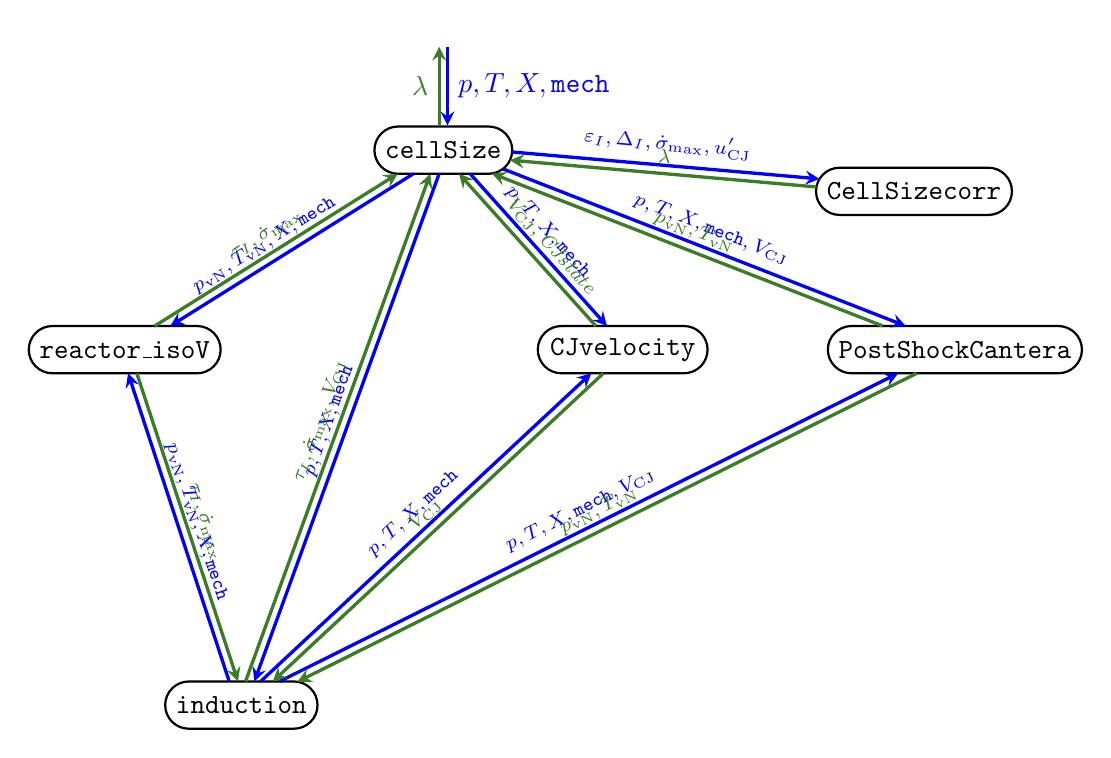
\begin{tikzpicture}[auto,>=stealth,node distance=2.5cm,
function/.style={
draw=black,
rounded rectangle,
minimum size=6mm,
font=\ttfamily,
thick,
}
]
\node [function,name path=cellSize]  (cellSize)  {cellSize};
\node[above=1cm of cellSize, name path=input]  (input){};
\node at (-5:6cm) [function,name path=CellSizecorr] (CellSizecorr){CellSizecorr};
\node at (-110:7.5cm) [function,name path=induction](induction){induction};
\node [function,above=4.2cm of induction.west,xshift=-0.5cm,name path=reactor](reactor){reactor\_isoV};
\node [function, right=4cm of reactor, name path=CJvelocity](CJvelocity){CJvelocity};
\node [function, right=1.5cm of CJvelocity, name path=PostShockCantera](PostShockCantera){PostShockCantera};


\draw[->,very thick, color=Blue]  ([xshift=1.5pt] input.south)  -- node {$p,T,X,\texttt{mech}$} ([xshift=1.5pt]cellSize.north);
\draw[->,very thick, color=OliveGreen]  ([xshift=-1.5pt]cellSize.north) -- node {$\lambda$} ([xshift=-1.5pt] input.south);
\foreach \i/\j/\k/\l in{%
									cellSize/CellSizecorr/{\varepsilon_I,\Delta_I,\dot{\sigma}_{\mathrm{max}},u'_{\mathrm{CJ}}}/{\lambda},
									cellSize/induction/{p,T,X,\texttt{mech}}/{\tau_I,\dot{\sigma}_{\mathrm{max}},V_{\mathrm{CJ}}},
									cellSize/PostShockCantera/{p,T,X,\texttt{mech},V_{\mathrm{CJ}}}/{p_{\mathrm{vN}},T_{\mathrm{vN}}},
									cellSize/CJvelocity/{$\hspace{-5pt}$p,T,X,\texttt{mech}}/{V_{\mathrm{CJ}},\mathit{CJstate}$\hspace{-10pt}$},
									cellSize/reactor/{$\hspace{-15pt}$p_{\mathrm{vN}},T_{\mathrm{vN}},X,\texttt{mech}}/{\tau_I,\dot{\sigma}_{\mathrm{max}}},
									induction/PostShockCantera/{p,T,X,\texttt{mech},V_{\mathrm{CJ}}}/{p_{\mathrm{vN}},T_{\mathrm{vN}}},
									induction/CJvelocity/{p,T,X,\texttt{mech}}/V_{\mathrm{CJ}},
									induction/reactor/{p_{\mathrm{vN}},T_{\mathrm{vN}},X,\texttt{mech}}/{\tau_I,\dot{\sigma}_{\mathrm{max}}}
									} 
		%\draw[very thick] (\i)  -- node[above] {\tiny{in: $\k$}} node[below] {\tiny{out: $\l$}} (\j) ;
		{
		\path [name path=in] let \p1 = ($(\j)-(\i)$) in (\i) ($(\i)!1.5pt!($(\i)+(-\y1,\x1)$)$) to +(\p1);
		\path [name path=out] let \p1 = ($(\i)-(\j)$) in (\j) ($(\j)!1.5pt!($(\j)+(-\y1,\x1)$)$) to +(\p1);
		\node [name intersections={of={\i} and in}] (tmp) at (intersection-1){};
		\draw [->, very thick, name intersections={of={\j} and in},color=Blue] (tmp.center) -- node[midway,sloped] {\scriptsize{$\k$}} (intersection-1);
		\node [name intersections={of={\j} and out}] (tmp) at (intersection-1){};
		\draw [->, very thick, name intersections={of={\i} and out},color=OliveGreen] (tmp.center) -- node[midway, sloped] {\scriptsize{$\l$}} (intersection-1);
		}
\end{tikzpicture}

\abk[zl]{$\lambda$}{Detonation cell size (m)}
\abk[p]{$p$}{Pressure (Pa)}
\abk[t]{$T$}{Temperature (K)}
\abk[m]{$\texttt{mech}$}{Name of chemical kinetic mechanism used in \emph{Cantera}}
\abk[x]{$X$}{Mixture mole fraction}
\abk[zt]{$\tau_{\mathrm{I}}$}{Induction time (s)}
\abk[p]{$p_{\mathrm{vN}}$}{von Neumann pressure (Pa)}
\abk[t]{$T_{\mathrm{vN}}$}{von Neumann temperature (K)}
\abk[v]{$V_{\mathrm{CJ}}$}{Detonation shock velocity (m/s)}
\abk[zs]{$\dot{\sigma}_{\mathrm{max}}$}{Maximum heat release rate (1/s)}
\abk[u]{$u'_{\mathrm{CJ}}$}{CJ particle velocity in a shock-attached frame (m/s)}
\abk[zd]{$\Delta_{\mathrm{I}}$}{Induction zone length (m)}
\abk[ze]{$\varepsilon_{\mathrm{I}}$}{Normalized activation energy of the induction process}%
\caption{Scheme of function calls, input and output variables for detonation cell size calculation}%
\label{scheme}%
\end{figure*}

%%%%%%%%% FUNCTIONS AND SUBFUNCTIONS %%%%%%%%%%%%%%%%%%%%%%%%%%%%%%%%%%%%%%%%%%%%%%%%%%%%%%%

\section{Functions and subfunctions}\label{fun}
All functions and subroutines necessary to approximate the detonation cell size of a certain combustable mixture are explained in detail in the next subsections. It must be stressed that almost all require the open source chemical kinetics software suite \emph{Cantera} to calculate mixture properties and equilibrium states. They were developed and tested using the MATLAB\textsuperscript{\circledR} module of \emph{Cantera~2.1.2} in combination with \emph{Python~3.4.2} and \emph{Numpy~1.9.1}. 

An overview of the structure of the entire calculation process is given in \autoref{scheme}. Input and output variables for individual functions are also depicted, symbolized by blue and green arrows, respectively.

Because of the modular approach to the challenge of computing various interdepending parameters, each function and subfunction solves a distinct purpose and can be used as a stand-alone calculation tool. For this reason, a major function like \texttt{cellSize} calls another major function, \texttt{induction}, to produce the induction time, but is also required to call various subfunctions of \texttt{induction} to obtain intermediate results which are not part of its final output.   

%%%%%%%%% CELLSIZE %%%%%%%%%%%%%%%%%%%%%%%%%%%%%%%%%%%%%%%%%%%%%%%%%%%%%%%%%%%%%%%%%%%%%%%%%

\subsection{\texttt{cellSize}}
To approximate the characteristic cell size, the \texttt{cellSize} function acts as the main function which takes the initial state of the mixture and the chosen kinetic mechanism $\texttt{mech}$ as input parameters.

\lstinputlisting[firstline=1,lastline=1]{../cellSize.m}

The initial state must consist of the static pressure $p$ in Pa, the temperature $T$ in K and $X$, which is either a column vector of mole fractions or a string listing all components according to \emph{Cantera} standards. This function calls all other functions and subfunctions to gather the required quantities needed by the approximation model that yields as a final result the approximated detonation length $\lambda$ in m.

The declaration is followed by:

\lstinputlisting[firstline=19,lastline=27]{../cellSize.m}
This code sections can be found in all functions that need to invoke a \emph{Cantera} phase for chemical calculations. Variable $\texttt{mech}$ is used to search for a corresponding mechanism in \emph{Cantera's} database. \emph{Cantera} converts its more verbose .cti files to .xml files via \emph{Python} before using them, therefore already converted mechanism files are preferred. For this reason, $\texttt{mech}$ may only consist of the name of the mechanism. For example, $\texttt{mech}=\texttt{'gri30'}$ is allowed, while $\texttt{mech}=\texttt{'gri30.xml'}$ would be searching for \texttt{'gri30.xml.xml'} and result in an error. 

Even though in principle all \emph{Cantera}-compatible kinetic mechanisms can be used, the latest 
recommendation for hydrogen-fueled detonations would be the mechanism developed by \citet{burke}, for 
its explicit consideration of high-pressure combustion.

The following code section calls the functions which calculate detonation properties of the given mixture:

\lstinputlisting[firstline=28,lastline=31]{../cellSize.m}
The \texttt{induction} function receives the exact same input values as \texttt{cellSize}. It starts the function chain to obtain the characteristic induction time $\tau_{\mathrm{I}}$ and is further described in \autoref{induction}. The next subfunction to be called by \texttt{cellSize} is \texttt{PostShockCantera}, fully explained in \autoref{post}. It solves the Hugoniot- and Rayleigh-equations\footnote{see \citep{deto_phen}} to obtain the von-Neumann conditions that are present directly after the shock front.

The next step is  the calculation of the non-dimensional global activation energy $\varepsilon_{\mathrm{I}}$, which is another stability parameter required by the approximation model for the characteristic cell size. Its use has been suggested by \citet{ng2,ng1}. To estimate its value, the method introduced by \citet[p.\,81]{schultz} is applied:

\lstinputlisting[firstline=32,lastline=43]{../cellSize.m}
The principle is to assume a global Arrhenius law in which the induction time depends on a global activation energy for the combustion reaction and the von-Neumann temperature of the mixture after the compression shock wave. In combination with the shock jump conditions and the assumption of a strong shock wave, inverting this relation leads to the bottom equation of the code section
\begin{equation*}
\varepsilon_{\mathrm{I}}= \frac{E_{\mathrm{I}}}{RT_{\mathrm{vN}}}=\frac{1}{T_{\mathrm{vN}}}\left(\frac{\ln \tau_{\mathrm{I}}^+ - \ln \tau_{\mathrm{I}}^-}{\frac{1}{T_{\mathrm{vN}}^+}-\frac{1}{T_{\mathrm{vN}}^-}}\right),
\end{equation*}
\abk[r]{$R$}{Ideal gas constant (J/(mol K))}%
where the superscripts $+$ and $-$ mark those induction time lengths and von-Neumann temperatures which result from calculations with detonation velocities altered by $\pm 1\%$. These values are therefore computed in advance by use of the already mentioned \texttt{PostShockCantera} subfunction, as well as the \texttt{reactor\_isoV} subfunction. The latter can be found in \autoref{reactor} and solves the equations of state in an ideal,  zero-dimensional and isochoric reactor.

The next section transforms the induction time into the required induction length:

\lstinputlisting[firstline=45,lastline=51]{../cellSize.m}
For this, the induction time is multiplied with the von-Neumann particle velocity in a shock attached reference frame. This velocity is also obtained by a shock jump condition, which relates the change in velocity across the shock wave to the change in density.

The last required input parameter for the model by \citet{ng1} is the	Chapman-Jouguet particle velocity in a shock-attached frame, $u'_{\mathrm{CJ}}$.

\lstinputlisting[firstline=53,lastline=55]{../cellSize.m}
It can be extracted from the CJ-state information that is part of the output of the \texttt{CJvelocity} subfunction, looked into in \autoref{cj}.

Finally, the the approximation polynom itself is called via the \texttt{cellSizeCorr} subfunction (see \autoref{corr}) and yields the desired characteristic length:
\lstinputlisting[firstline=57,lastline=58]{../cellSize.m}

%%%%%%%%%%% INDUCTION %%%%%%%%%%%%%%%%%%%%%%%%%%%%%%%%%%%%%%%%%%%%%%%%%%%%%%%%%%%%%%%%%%%%%%

\subsection{\texttt{induction}}\label{induction}
The \texttt{induction} function serves as a stand-alone calculation tool to obtain the characteristic induction time $\tau_{\mathrm{I}}$ of a Chapman-Jouguet detonation. Its input requirements are the same as for the \texttt{cellSize} function.

\lstinputlisting[firstline=1,lastline=1]{../induction.m}

The first code block computes and displays the detonation velocity $V_{\mathrm{CJ}}$ via \texttt{CJvelocity}: 

\lstinputlisting[firstline=25,lastline=29]{../induction.m}
Following this, like in \texttt{cellSize}, the von-Neumann state is provided by \texttt{PostShockCantera}: 

\lstinputlisting[firstline=31,lastline=33]{../induction.m}

The last step is the use of the ideal isochoric reactor model in \texttt{reactor\_isoV}, taking the von-Neumann state as input parameters:

\lstinputlisting[firstline=35,lastline=36]{../induction.m}
In this case, not only $\tau_{\mathrm{I}}$ is calculated, but also the maximum heat release rate $\dot{\sigma}_{\mathrm{max}}$. The latter has has a dimension of 1/$s$, so its inverse value is used in the model of \citet{ng1} to express the characteristic time scale of the heat release, i.e. the reaction time, which is another required stability parameter.

%%%%%%%%%%% CJ-VELOCITY %%%%%%%%%%%%%%%%%%%%%%%%%%%%%%%%%%%%%%%%%%%%%%%%%%%%%%%%%%%%%%%%%%%%

\subsection{\texttt{CJvelocity}}\label{cj}
The \texttt{CJvelocity} function iteratively solves the one-dimensional continuity, momentum and energy equations for a CJ detonation at given initial pressure and temperature. Output parameters are the CJ velocity and the \texttt{CJstate} structure consisting of the values of pressure, temperature, mole fractions and particle velocity at the CJ plane of the detonation (which, per definition, is located where the local Mach number is $Ma=1$). \abk[m]{$\mathit{Ma}$}{(local) Mach number}

\lstinputlisting[firstline=1,lastline=1]{../CJvelocity.m}
The following code section is excerpted almost unaltered (apart from certain syntax difference between Fortran95 and MATLAB\textsuperscript{\circledR} code) from the NASA \emph{Chemical Equilibrium  with Applications} toolbox (\emph{CEA}, \citep{cea}), which is freely available. Its mathematical foundations, which can be inspected in the \emph{CEA} manual, are based on the solution of the CJ detonation state relations by a Newton-Raphson iteration, as proposed by \citet{zeleznik}. 

Chemical equilibrium is calculated for assumed values of $p_{\mathrm{CJ}}$ and $T_{\mathrm{CJ}}$. Results are then used to solve the momentum and energy relations across a CJ detonation, using the residuals as an adjustment parameter and convergence criteria for the original estimates.
\abk[p]{$p_{\mathrm{CJ}}$}{Pressure in the CJ plane (Pa)}
\abk[T]{$T_{\mathrm{CJ}}$}{Temperature in the CJ plane (K)}

The first challenge is to find suitable values for an initial guess of $p_{\mathrm{CJ}}$ and $T_{\mathrm{CJ}}$. This is done in two steps:

\lstinputlisting[firstline=36,lastline=49]{../CJvelocity.m}
While $p_{\mathrm{CJ}}$ is approximated as $\approx 15\,p_0$, the first guess for $T_{\mathrm{CJ}}$ is calculated by finding the adiabatic flame temperature for a fixed equilibrium enthalpy. This assumption is based on the relatively small range of possible solutions for the pressure ratio in a detonation as is argued by \citet{zeleznik}. 

Additional refinement of the initial conditions is undertaken in the following loop:

\lstinputlisting[firstline=51,lastline=64]{../CJvelocity.m}
Here, the initial values are further improved using a method of successive substitutions\footnote{see \citep{zeleznik}}. These recursion formulas are used three times, as in the original \emph{CEA} tool. Over the course of this, the \texttt{partDeriv} subfunction, which is included at the end of \texttt{CJvelocity}, is used for the first time to calculate partial derivatives necessary to obtain the correct values for the equilibrium isentropic exponent $\gamma_s$ and equilibrium isobaric heat capacity $c_{p,\mathrm{eq.}}$. The function is further discussed at the end of this subsection.
\abk[zc]{$\gamma_s$}{equilibrium isentropic exponent} 
\abk[c]{$c_{p,\mathrm{eq.}}$}{equilibrium specific heat capacity at constant pressure (J/(kg K))} 

The next section of code holds the main iteration loop:

\lstinputlisting[firstline=66,lastline=105]{../CJvelocity.m}
As before, a gas state is introduced and brought to equilibrium according to the current values of $p_{\mathrm{CJ}}$ and $T_{\mathrm{CJ}}$. Mean molar mass and partial derivatives of this gas state can be calculated using the aforementioned \texttt{partDeriv} function. Results are then used in the iteration equations\footnote{Which make use of several abbreviations, see again the \emph{CEA} manual or \citep{zeleznik} for a detailed explanations}. Residuals \texttt{x1} and \texttt{x2}, corresponding to $p_{\mathrm{CJ}}$ and $T_{\mathrm{CJ}}$, respectively, are taken into account for the correction of the initial guess. Since the equations are solved for $\ln \left(\frac{p_{\mathrm{CJ}}}{p_0}\right)$ and $\ln \left(\frac{T_{\mathrm{CJ}}}{T_0}\right)$, these corrections must be done via an exponential function. The \texttt{delta} parameter that is additionally applied is supposed to suppress divergent behavior of the solution.

If the solution does not converge within 8 iterations, the iteration loop is aborted. Otherwise, $V_{\mathrm{CJ}}$ is calculated from $u'_{\mathrm{CJ}}$ through the mass equation and other CJ properties are saved in \texttt{CJstate}.

The last part of \texttt{CJvelocity} is the already mentioned \texttt{partDeriv} subfunction. Its output variables are the equilibrium isentropic exponent $\gamma_s$, the equilibrium isobaric heat ratio $c_{p,\mathrm{eq.}}$ and the partial derivatives $\left(\frac{\partial \ln v}{\partial \ln p}\right)_T$ and $\left(\frac{\partial \ln v}{\partial \ln T}\right)_p$.

\lstinputlisting[linerange={108-108,116-145}]{../CJvelocity.m}
This part is not included in the original \emph{CEA} code since it uses its own chemical equilibrium solver, and the \emph{Cantera} software used in this work does not provide an interface to calculate partial derivatives on its own. 

Another problem arises from the fact that \emph{Cantera} only offers \emph{frozen} (i.e., fixed mixture composition) values for thermodynamic properties like $c_p$, resulting from the weighted sum of the properties of each component of a mixture. But according to \citet{wood}, equilibrium values for speed of sound and for other thermodynamic properties should be used. 

The equilibrium specific heat ratio $c_{p,\mathrm{eq.}}$ is therefore approximated as 
\begin{equation*}
c_{p,\mathrm{eq.}}=\frac{h_{\mathrm{eq.}}(T_0+\Delta T)-h_{\mathrm{eq.}}(T_0-\Delta T)}{2 \Delta T},
\end{equation*}
using a central difference scheme with the equilibrium enthalpy and a step width of $\Delta T=1\cdot 10^{-6}$\;K.

The isentropic exponent $\gamma_s$ is another important parameter. Coming from the definition of the speed of sound as it is made by \citet{zeleznik}, its most general definiton is
\begin{equation*}
\gamma_s =  \left(\frac{\partial \ln p}{\partial \ln \rho}\right)_s.
\end{equation*}
\citet{cea} use the Bridgman tables to rearrange this to achieve the expression
\begin{equation*}
\gamma_s = - \frac{c_{p,\mathrm{eq.}}}{c_{v,\mathrm{eq.}}}\left(\frac{\partial \ln v}{\partial \ln p}\right)_T^{-1}.
\end{equation*}
\abk[v]{$v$}{Specific volume (m$^3$/kg)}
From the ideal gas law, $\left(\frac{\partial \ln v}{\partial \ln p}\right)_T$ is equal to $-\left(\frac{\partial \ln M_{\mathrm{mean}}}{\partial \ln p}\right)_T-1$. As can be seen easily, if the last partial derivative is zero, we will obtain the more familiar equation $\gamma_s =  \frac{c_p}{c_v}$. However, for a fast reacting mixture in general and a highly pressure dependent detonation combustion especially, the mean molar mass of the components \emph{will} change with respect to pressure perturbations, and it is therefore necessary to use the more general expression above\footnote{The impact of this measure is generally small, but can be important under certain circumstances (especially for low pressures), as is shown in the original article by \citet[Table 7]{zeleznik}}.

For that reason, the partial derivatives $\left(\frac{\partial \ln v}{\partial \ln p}\right)_T$ and $\left(\frac{\partial \ln v}{\partial \ln T}\right)_p$  are approximated using a central difference scheme for a step width of $\Delta p=1\cdot 10^{-8}$\;Pa and $\Delta T=1\cdot 10^{-6}$\;K respectively.\footnote{The second one can be used to replace $c_v$, after some more rearrangements according to the Bridgman tables, see \citep{cea}}

\subsection{\texttt{PostShockCantera}}\label{post}

The purpose of the \texttt{PostShockCantera} function is to calculate the post-shock (von-Neumann) state of $p$ and $T$ from an already solved CJ relation.
 
\lstinputlisting[firstline=1,lastline=1]{../PostShockCantera.m}
It makes use of the internal MATLAB\textsuperscript{\circledR} function \texttt{fzero} to solve a functional composed of the Hugoniot- and Rayleigh-equation for the density $\rho$. 
\abk[zr]{$\rho$}{Density (kg/m$^3$)}

\lstinputlisting[firstline=34,lastline=46]{../PostShockCantera.m}
The so obtained $\rho$ is taken to solve the Rayleigh equations for pressure and energy, which then can be used by \emph{Cantera} to calculate the corresponding von-Neumann state.

The last code section consists of a function for the aforementioned functional. It calculates the intersection of the Rayleigh- and Hugoniot-equations by iteration.

\lstinputlisting[linerange={40-40,47-66}]{../PostShockCantera.m}
An initial guess of $\rho$ is made, and the difference of the resulting values for $p$ by each corresponding equation is taken as the error to be minimized. 

Care must be taken when choosing the initial guess for $\rho$. Experience has shown that the minimization of the functional can result in convergence for values of $\rho$ which are very close or equal to the initial value of $\rho_0$. Since we expect a drastic increase in density for the post-shock state in most cases, these incorrect results can usually be identified easily. A solution is to further increase either the value for the initial guess of $\rho$ (which, for this reason, is already 15 by default) or the penalty for convergence values close to the initial value, as described in the comment at the end of the function. However, in some cases it might be also necessary to reduce the default value. This is mostly the case for very weak shocks, resulting for example from very rich or diluted mixtures.  

\subsection{\texttt{reactor\_isoV}}\label{reactor}
The function \texttt{reactor\_isoV} solves the ordinary differential equations for the chemical kinetics (\texttt{mech}) of a specific mixture ($X$) in a specific initial state ($p,T$), assuming a non-dimensional constant volume combustion inside the reaction zone. Output values are the induction time $\tau_{\mathrm{I}}$, i.e., time that passes until autoignition of the mixture, and the maximum heat release rate $\dot{\sigma}_{\mathrm{max}}$, which is also called the maximum thermicity. 

\lstinputlisting[firstline=1,lastline=1]{../reactor\string_isoV.m}
According to \citet[p. 195]{deto_phen}, the error resulting from the simplified constant-volume model can be neglected for an assumed simple linear dependence between the ZND detonation zone length $\Delta_{\mathrm{I}}$ and the detonation cell size $\lambda$.

\lstinputlisting[firstline=24,lastline=36]{../reactor\string_isoV.m}
The first lines only derive initial values for the temperature, thermicity and the mass fraction of each species from the submitted initial state of the mixture. After this, options for the later used MATLAB\textsuperscript{\circledR} function \texttt{ode15s} regarding tolerance values for convergence are set up. The time scale in which the model is run must be adjusted to the needs of the specific mixture. This mostly depends on the fuel that is used. A run time which is too short might push the point of ignition out of scope, while an unnecessary long run time wastes processing time. 

The actual solving of the ODE-system is accomplished in the next lines:

\lstinputlisting[firstline=38,lastline=42]{../reactor\string_isoV.m}
The \texttt{ode15s} function solves the ordinary differential equations for an isochoric reactor, which are are defined at the end of the file in a separate function named \texttt{isoVsigma\_ode}. The results are two arrays, containing the time steps and the values of the solved variables (i.e., $T$, $X$ and $\dot{\sigma}$). $\dot{\sigma}_{\mathrm{max}}$ is simply the maximum of all values of $\dot{\sigma}$\footnote{The solver for for the ordinary differential equation per default integrates the solutions over time. Therefore, to obtain the actual thermicity, which is a time rate of dimension $\mathrm{s}^{-1}$, the gradient of the solution has to be taken.}.

The determination of $\tau_{\mathrm{I}}$ is done according to the following definition:

\lstinputlisting[linerange={44-47}]{../reactor\string_isoV.m}
This means that the point of ignition is defined as the moment of steepest ascent in temperature. Other definitions are possible and also common; adjustments can easily be made.

The following function \texttt{isoVsigma\_ode} consists of the right hand sides of the ordinary differential equations for a constant-volume combustion reactor. 

\lstinputlisting[firstline=59,lastline=77]{../reactor\string_isoV.m}
The change of species concentration is calculated by solving the reaction kinetics through \emph{Cantera}. Temperature changes can be directly related to the increase or decrease of the specific internal energy. The definition of thermicity for an ideal gas
\begin{equation*}
\dot{\sigma}=\sum_{i=1}^{N_s} \left(\frac{M_{\mathrm{mean}}}{M_i}-\frac{h_i}{c_p T}\right)\frac{\mathrm d y_i}{\mathrm d t}
\end{equation*}
is derived by \citet{kao}.
\abk[m#]{$M$}{Molar mass (kg/mol)}
\abk[h]{$h$}{Specific enthalpy (J/kg)}
\abk[n]{$N_s$}{Total number of species}
\abk[t~]{$t$}{Time (s)}
\abk[y]{$y$}{Normalized reaction rate}

\subsection{\texttt{cellSizeCorr}}\label{corr}
This function only includes the suggested polynomial factors to relate $\Delta_{\mathrm{I}}$ to $\lambda$ by the model of \citet{ng1}.

\lstinputlisting{../cellSizeCorr.m}
The aforementioned stability parameters $\varepsilon_{\mathrm{I}}$ and $\dot{\sigma}_{\mathrm{max}}$, as well as the particle velocity $u'_{\mathrm{CJ}}$, are also applied.

\section{Prospects}

Results of the described model have been compared to various available experimental data for detonation cell sizes of H$_2$-O$_2$ and H$_2$-Air mixtures. Examples of these comparisons can be seen in \autoref{o2} and \autoref{air}. For the examined ranges of initial parameters, an overall good agreement is observed. 

However, experimental data for higher pressures is sparse, while divergence between experimental results for lower pressures is high. An increasing influence of the choice of the applied kinetic mechanism can be recognized for very lean and very rich mixtures.

Although accuracy within a magnitude of $\approx 1$\,mm seems to be possible for H$_2$-O$_2$ mixtures, H$_2$-Air mixtures already only seem to provide an accuracy within a magnitude of $\approx 10$\,mm, which can prove to be too much for stability considerations.

Moreover, the assumption of a constant volume reactor to calculate the induction time and thermicity is a simplification of the actual detonation reactions. Comparisons of the CJ temperatures calculated by the CEA code and by the constant volume reactor show a discrepancy with a magnitude of several 100\,K. As has been stated in \autoref{reactor}, differences in results for $\lambda$ can be mostly neglected for a simple linear dependence between detonation zone length and cell size. But since the polynomial parameters of the model also depend on $\varepsilon_{\mathrm{I}}$, $\Delta_{\mathrm{I}}$ and $\dot{\sigma}_{\mathrm{max}}$, which themselves depend on induction time and heat release, strictly speaking, this assumption is not valid. Therefore, the use of a genuine ZND reactor model should be considered. An example for such a reactor is provided by \citet{kao} as part of the shock-detonation-toolbox. 

\begin{figure*}[h]%
\centering%
\includegraphics[width=\textwidth]{VergleichO2}
\caption{Comparison of numerical and experimental results for H$_2$-O$_2$ mixtures}
\label{o2}
\vspace{1cm}
\includegraphics[width=\textwidth]{VergleichAir}
\caption{Comparison of numerical and experimental results for H$_2$-Air mixtures}
\label{air}
\end{figure*}

% LITERATURVERZEICHNIS %%%%%%%%%%%%%%%%%%%%%%%%%%%%%%%%%%%%%%%%%%%%%%%%%%%%%%%%%%%%%%%%%%%%%
%\clearpage
\phantomsection
\addcontentsline{toc}{section}{References} % Literaturverzeichnis ins Inhaltsverzeichnis schreiben
\nocite{*}
\bibliographystyle{plainnat} % Literaturverzeichnis Stil
{\scriptsize
\bibliography{literatur/literature} % Quellendatenbank
}
%% Anh�nge %%%%%%%%%%%%%%%%%%%%%%%%%%%%%%%%%%%%%%%%%%%%%%%%%%%%%%%%%%%%%%%%%%%%%%%%%%%%%%%%%
%\appendix
% ==> F�lle diesen Platz mit neuen Dateien oder Inhalten f�r den Anhang
\end{multicols}

\end{document}